\section{Non-Abelian Gauge Theory, Yang-Mills \& QCD}
For the remaining lectures of this class, we can discuss some aspects of non-Abelian gauge theory, touching on some ideas of Yang-Mills and QCD. This is in some sense the one missing puzzle piece we need to construct all QFTs (well, other than perhaps gravity).

Non-abelian gauge fields arise in a number of settings:
\begin{itemize}
    \item Particle physics: Electroweak sector, QCD.
    \item Condensed Matter: Non-Abelian quantum hall states (2+1d QFT).
    \item Quantum Gravity: $\mathcal{N}=4 SU(N)$ super Yang-Mills; our best understood models of gauge-gravity duality.
    \item Also: Weakly coupled RG fixed points in 3+1d (Bankz-Zaks fixed points).
    \item Mathematical perspective: Connections on fiber bundles.
\end{itemize}

\subsection{A simple QFT with $U(N)$ symmetry}

We'll follow an approach similar to QED, starting with a theory that has a \emph{global} non-Abelian symmetry. Specifically, we consider $N$ Dirac fermions:
\begin{equation}
    S = \sum_{i=1}^N \int d^4x \bar{\psi}_i(i\slashed{\p} - m)\psi_i
\end{equation}
These Dirac fermions have two indices $\psi_{i\alpha}$; $\alpha$ is the usual spinor index we usually suppress, $i$ is now the flavour, or colour index, which ranges from $i = 1, \ldots N$.

What are the symmetries of this model? We consider:
\begin{equation}
    \vec{\psi} = \m{\psi_1 \\ \psi_2 \\ \vdots \\ \psi_N} \to U\psi
\end{equation}
and:
\begin{equation}
    \bar{\psi}^\dag \to \psi^\dag U^\dag
\end{equation}
which implies:
\begin{equation}
    \bar{\psi} \to \psi^\dag U^\dag \gamma_0 = \bar{\psi}U^\dag
\end{equation}
in order for this action to be invaraint, we require that:
\begin{equation}
    \bar{\psi}\psi \to \bar{\psi}U^\dag U \psi = \bar{\psi}U^\dag U \psi
\end{equation}
which requires that:
\begin{equation}
    U^\dag U = \II
\end{equation}
in other words, $U \in U(N)$, i.e. the group of unitary $N \times N$ matrices. This is a continuous symmetry.

How many symmetries is this? It's easier to think about unitary matrices as matrix exponentials:
\begin{equation}
    U = e^{iT}
\end{equation}
where $U^\dag = e^{-iT^\dag}$ and $U^{-1} = e^{-iT}$, so in order for $U \in U(N)$ we require $T^\dag = T$, i.e. $T$ is Hermitian.

This is much easier to count; $T$ is Hermitian so on the diagonal we have all real numbers, $t_{ii} \in \RR$ and for off diagonals we have $t_{ij} = t_{ji}^*$. This gives us $N^2$ parameters/symmetries (each matrix element provides one real parameter). Compare this to the $U(1)$ case, where we had a single symmetry/single complex number/phase.

Let $T_a, a = 1, \ldots, N^2$ be a basis of generators of the algebra $\mathfrak{u}(N)$. Now, we can write $U \in U(N)$ as $e^{i\lambda^a T_a} = U$, with $\lambda^a \in \RR$ real parameters.

After $U(1)$, the next simplest example is $U(2)$. We consider a set of 4 $2\times 2$ Hermitian matrices $\mathfrak{u}(2)$. We then have $T_a = \set{\II, \sigma_i}$, so then;
\begin{equation}
    U = e^{i\lambda_0}e^{i\lambda_i\sigma^i} \in U(2)
\end{equation}
So we notice that the identity part actually commutes with the rest! So, we can actually break up the group. Note that $\II$ has a pure trace and $\sigma_i$ are traceless, so the exponential has determinant 1. Thus we can write:
\begin{equation}
    U(2) = U(1) \times SU(2)
\end{equation}
And more generally:
\begin{equation}
    U(N) = U(1) \times SU(N)
\end{equation}
the $SU(N)$ part contains the Non-Abelian character of the group:
\begin{equation}
    [T_a, T_b] \neq 0
\end{equation}
We then note that:
\begin{equation}
    [T_a, T_b]^\dag = [T_b^\dag, T_a^\dag] = [T_b, T_a] = -[T_a, T_b]
\end{equation}
using that the $T_a$ are Hermitian, This implies that the commutator is anti-Hermitian:
\begin{equation}
    [T_a, T_b] = if_{ab}^{\sp \sp c}T_c
\end{equation}
the $f_{ab}^{\sp \sp c}$ are known as structure factors. For $SU(2)$, we have:
\begin{equation}
    [\sigma_i, \sigma_j] = i\e_{ijk}\sigma_k
\end{equation}
so the structure factor of $SU(2)$ is $\e_{ijk}$.

\subsection{Noether Currents for $U(N)$ symmetry}
To find the associated Noether currents for these symmetries, let us perform:
\begin{equation}
    U(x) = e^{i\lambda^a(x)T_a} \approx 1 + i\lambda^a(x)T_a + \ldots
\end{equation}
The change in the action then is:
\begin{equation}
    S \to S' = \int d^4x\bar{\psi}U^{-1}(x)(i\slashed{\p} - m)U(x)\psi
\end{equation}
The change in the action only comes from the term where the derivative hits $U(x)$, so:
\begin{equation}
    \delta S = S' - S = -\int d^4x \bar{\psi}\gamma^\mu \p_\mu \lambda^a(x)T_a \psi = -\int d^4x \p_\mu \lambda^a(x)\psi \gamma^\mu T_a\psi
\end{equation}
So we can identify:
\begin{equation}
    j^\mu_a = \psi \gamma^\mu T_a \psi
\end{equation}
for $a = 1, \ldots, N^2$ as the Noether currents.

\subsection{Gauging the symmetry}
Let us try to make this theory more interesting by ``gauging'' the $U(N)$ symmetry, in other words turning the global $U(N)$ symmetry into a local $U(N)$ symmetry. The problem comes in with the kinetic term (the mass term is already invariant - hence we saw it dropped out of the current). Let's try to make the kinetic term gauge invariant by adding a term $j^\mu_a A^a_\mu$ to $\mathcal{L}$:
\begin{equation}
    j^\mu_a A^a_\mu = A_\mu^a \bar{\psi}\gamma^\mu T_a \psi = \bar{\psi}\gamma^\mu A^a_\mu T_a \psi \equiv \bar{\psi}\gamma^\mu A_\mu^a T_a \psi
\end{equation}
where we define a Hermitian matrix $A_\mu$. The action then becomes:
\begin{equation}
    \begin{split}
        S = \int \bar{\psi}i\gamma^\mu(\p_\mu + iA_\mu)\psi &\to \int \bar{\psi}i\gamma^\mu U^{-1} (\p_\mu + iA_\mu')U\psi
        \\ &= \int \bar{\psi}i\gamma^\mu [U^{-1}\p_\mu U + U^{-1} i A_\mu' U]\psi + \bar{\psi}i\slashed{\p}\psi
    \end{split}
\end{equation}
We wish for this to be Gauge invariant, which requires:
\begin{equation}
    U^{-1}\p_\mu U + U^{-1} i A_\mu' U = iA_\mu
\end{equation}
So:
\begin{equation}
    A_\mu \to A_\mu' = UA_\mu U^{-1} + iU(U^{-1}\p_\mu U)U^{-1} = UA_\mu U^{-1} + i(\p_\mu U)U^{-1}
\end{equation}
Now noticing that:
\begin{equation}
    0 = \p_\mu(UU^{-1}) = \p_\mu U U^{-1} + U\p_\mu U^{-1}
\end{equation}
(and a similar relation holds for $\p(U^{-1}U)$) we can write:
\begin{equation}
    A_\mu \to A_\mu' = UA_\mu U^{-1} - iU\p_\mu U^{-1} = U(A_\mu - i\p_\mu)U^{-1}
\end{equation}
To check that we've done this right, we can recall in the $U(1)$ case that we had $U = e^{i\lambda}$ (a scalar) for which:
\begin{equation}
    A_\mu \to A_\mu - \p_\mu \lambda
\end{equation}
which is consistent with our general formula.

The transformation of $A$ allows us to build a covariant derivative:
\begin{equation}
    \begin{split}
        D_\mu \psi = (\p_\mu + iA_\mu)\psi &\to [\p_\mu + i(U(A_\mu - i\p_\mu)U^{-1})]U\psi
        \\ &= U\p_\mu \psi + (\p_\mu U)\psi + i UA_\mu \psi + U(\p_\mu U^{-1})U\psi 
        \\ &= U\p_\mu \psi + (\p_\mu U)\psi + i UA_\mu \psi + -\p_\mu U \psi
        \\ &= U(\p_\mu + iA_\mu)\psi 
        \\ &= UD_\mu \psi
    \end{split}
\end{equation}
With this building block, it is easy to build gauge-invariant actions:
\begin{equation}
    S = \int d^4x \bar{\psi}(i\slashed{D} - m)\psi
\end{equation}
if we hide the flavour indices, looks just like QED again.

\subsection{Building up a field strength}
There is a slight subtlety - can we build a gauge invariant term out of $A^a_\mu$ only? We may be tempted to consider the field strength, as we did in QED:
\begin{equation}
    \tilde{F}^a_{\mu\nu} = \p_\mu A^a_\nu - \p_\nu A^a_\mu
\end{equation}
But this turns out not to work:
\begin{equation}
    \begin{split}
        \tilde{F}^a_{\mu\nu}T_a \equiv \tilde{F}_{\mu\nu} = \p_\mu A_\nu - \p_\nu A_\mu &\to \p_\mu (U(A - i\p_\nu)U^{-1}) - (\mu \leftrightarrow \nu)
        \\ &= U^{-1}(\p_\mu A_\nu - \p_\nu A_\mu)U + [\p_\mu U A_\nu U^{-1} - i\p_\mu U \p_\nu U^{-1} + UA_\nu \p_\mu U^{-1} - (\mu \leftrightarrow \nu)]
        \\ &= U^{-1}\tilde{F}_{\mu\nu}U + + [\p_\mu U A_\nu U^{-1} - i\p_\mu U \p_\nu U^{-1} + UA_\nu \p_\mu U^{-1} - (\mu \leftrightarrow \nu)]_*
    \end{split}
\end{equation}
so we have unfortunately a bit of a mess. To find the correct expression for $F$, let us find something that is 0 for a pure gauge configuration:
\begin{equation}
    \alpha_\mu = -iU\p_\mu U^{-1}
\end{equation}
which we can see is gauge equivalent to $A_\mu = 0$. If $F$ is gauge invariant, it better be zero when we hand it the above.

Let's compute our naive guess for this object - does it vanish?
\begin{equation}
    \begin{split}
        \p_\mu \alpha_\nu - \p_\nu \alpha_\mu &= -i\p_\mu U \p_\nu U^{-1} - (\mu \leftrightarrow \nu)
        \\ &= iU\p_\mu U^{-1} U \p_\nu U^{-1} - (\mu \leftrightarrow \nu)
        \\ &= -i(\alpha_\mu \alpha_\nu - \alpha_\nu \alpha_\mu)
    \end{split}
\end{equation}
This doesn't vanish, but if we take the difference we get something that does equal zero for a pure gauge configuration:
\begin{equation}
    \boxed{F_{\mu\nu} \equiv \p_\mu A_\nu + iA_\mu A_\nu - (\mu \leftrightarrow \nu)}
\end{equation}
this vanishes if $A_\mu = \alpha_\mu = -i U\p_\mu U^{-1}$ a pure gauge. Spelling the above, nonlinear field strength out:
\begin{equation}
    F_{\mu\nu} = \p_\mu A_\nu - \p_\nu A_\mu + i[A_\mu, A_\nu]
\end{equation}
for which the commutator vanishes if we have an Abelian gauge theory. Let's see if this field strength is indeed gauge invariant:
\begin{equation}
    \begin{split}
        F_{\mu\nu} &\to U(\p_\mu A_\nu - \p_\nu A_\mu)U^{-1} + [\ldots]_* + [iU(A_\mu - i\p_\mu)U^{-1}U(A_\nu - i\p_\nu)U^{-1} - (\mu \leftrightarrow \nu)]
    \end{split}
\end{equation}
Let's look at the third term; we have a $U(A_\mu A_\nu - A_\nu A_\mu)U^{-1}$ which teams up with the first term to give us the field strength. The other contributions from it cancel out perfectly what is in $*$:
\begin{equation}
    \begin{split}
        &U\p_\mu U^{-1}UA_\nu U^{-1} + UA_\mu \p_\nu U^{-1} - iU\p_\mu U^{-1} U \p_\nu U^{-1} - (\mu \leftrightarrow \nu)
        \\ &= -\p_\mu U A_\nu U^{-1} + U_A\mu \p_\nu U^{-1} - i\p_\mu U \p_\nu U^{-1} - (\mu \leftrightarrow \mu)
    \end{split}
\end{equation}
Thus the transformation of the field strength is:
\begin{equation}
    F_{\mu\nu} \to U(\p_\mu A_\nu + iA_\mu A_\nu - (\mu \leftrightarrow \nu))U^{-1} = UF_{\mu\nu}U^{-1}
\end{equation} 
So we've improved things, but it is not quite gauge invariant. However, by our construction we know $F_{\mu\nu}$ only transforms via unitary conjugation/a basis transformation, so we know that \emph{traces} and higher powers of it are fully gauge invariant:
\begin{equation}
    \Tr(F_{\mu\nu}), \Tr(F_{\mu\nu}F_{\alpha\beta}), \Tr(FFF\ldots F), \Tr(F\ldots DF\ldots F)
\end{equation}
However we can't put these into the action directly because they have free Lorentz indices. The simplest LI term is then the trace of $F$ contracted with itself:
\begin{equation}
    \Tr(F_{\mu\nu}F^{\mu\nu})
\end{equation}
Finally, we arrive at our QCD action:
\begin{equation}
    S = \int \bar{\psi}(i\slashed{D} - m) - \frac{1}{4g^2}\Tr(F_{\mu\nu}F^{\mu\nu})
\end{equation}
in QCD, the fermions $\psi_i$ are quarks and the gauge fields $A_\mu^a$ are gluons. It looks deceptively similar to QED (fermions, gauge fields, a dimensionless coupling $g$), but it as a crucial difference. Namely, even without the fermions (i.e. the absence of matter), the gauge sector is interacting/non-linear. It is sometimes called ``pure glue''. Even the theory of ``pure glue'' is highly interacting/non-trivial! It is called Yang-Mills theory:
\begin{equation}
    S_{\text{YM}} = -\frac{1}{4g^2}\int d^4x \Tr(F_{\mu\nu}F^{\mu\nu})
\end{equation}
which contains terms/diagrams:

\begin{center}
    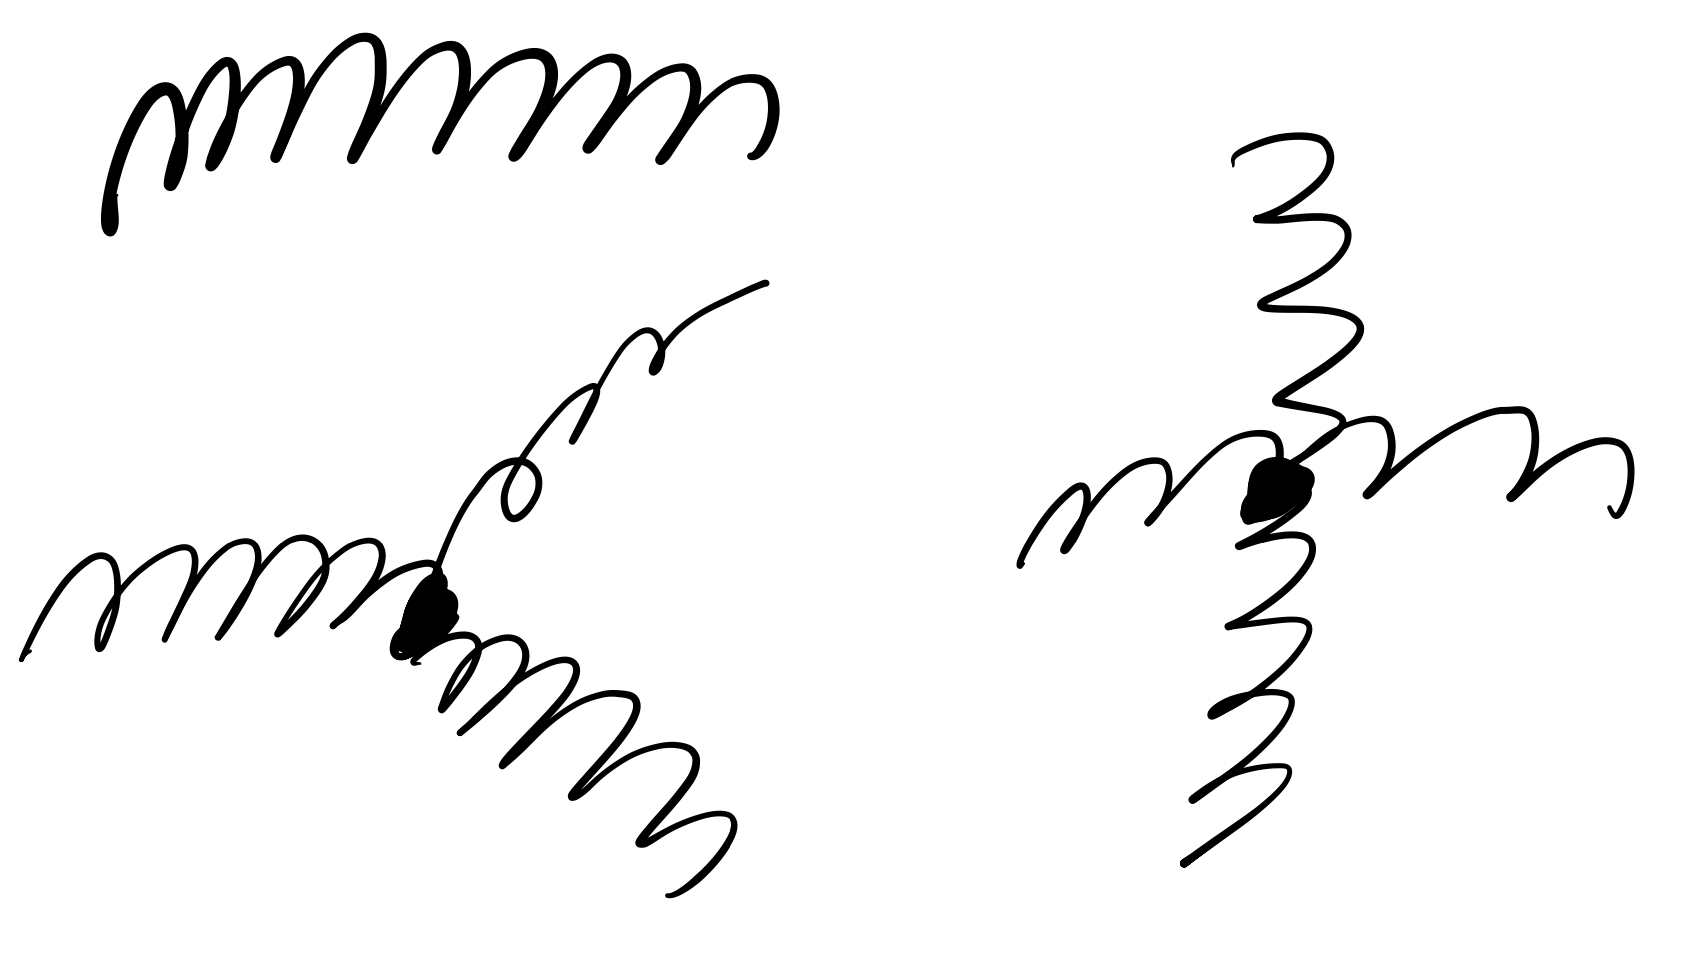
\includegraphics[scale=0.35]{Lectures/Images/lec16-gluons.png}
\end{center}

and is an unsolved theory. You'll get a million dollars/a Millenium prize if you can figure out if it confines at low energies - good luck. We can treat it with RG, however, and this approach has been met with success (though perturbation theory breaks down in the strongly interacting regime - this has motivated the bootstrap approach to QFT).

Next week, we will quantize this theory, following a similar procedure as we did for the photon, with one small change.